% Paper 11 (TN Holdings), DRAFT 4 (the workplace reading of draft 3 applied, 2026-11-24), home, 2026-11-22 (owner 23:29 JST "始めて"). Built from notes/paper11/OUTLINE.md
% and the committed records named beside each number; every number is quoted from those records (README and score
% files) and is to be checked one by one against them before release (tools/check_readme_numbers.py and a home VS
% reading). Figures: notes/paper11/figures.py. psf-os 0.3.3 (which includes 0.3.2) is to be released with this paper.
\documentclass[10pt,a4paper]{article}
\usepackage[margin=2.2cm]{geometry}
\usepackage{amsmath,amssymb}
\usepackage{booktabs}
\usepackage{array}
\usepackage{graphicx}
\usepackage[hidelinks]{hyperref}
\usepackage{float}
\input{glyphtounicode}
\pdfgentounicode=1
\setlength{\parskip}{4pt}
\setlength{\parindent}{0pt}
\sloppy
\newcommand{\pending}[1]{\textbf{[PENDING: #1]}}
\newcommand{\ket}[1]{|#1\rangle}

\title{Where a Qubit Waits:\\ Rules for Real-Time Control from Declared Device Tests on IBM Heron}
\author{TN Holdings\\ \small contact: \texttt{love.os.architect@proton.me}}
\date{Draft 4, 24 November 2026}

\begin{document}
\maketitle

\begin{abstract}
A circuit that measures in the middle and acts on the result at once loses part of what it keeps while it waits. Paper 10
of this series showed that such real-time control on IBM Heron devices can get closer to the exact answer than any
correction of the uncontrolled circuit. This paper asks what an operating layer should do with the waits. Every test
was declared in git before its device record was fetched; every comparison that decides a rule was made inside one
job; every shot was counted, and no error mitigation, post-selection or fitted noise model was used. Nine declared runs (eleven tests; the decoy and loopvar tests shared one session) were sent in eight charged sessions
on three devices (ibm\_marrakesh, ibm\_fez, ibm\_kingston; 706 s charged; 11 declared predictions, all held; a prediction was declared only where an earlier device record
grounded it, and over the series 20 of 68 failed, all on paper 10's nights). Four rules came out. (1) A qubit that waits in $\ket{1}$ keeps more if it is turned to $\ket{0}$ for the wait and back
after: $+0.039$ (2 SE 0.005) on iterative phase estimation (IPE) at $n=4$, $+0.031$ to $+0.039$ at $n = 4,5,6$ on
another calibration, $+0.029$ and $+0.052$ on two further devices; fencing it so that it waits in $\ket{1}$ instead of a
superposition read SAME WITHIN ERROR ($-0.004$, 2 SE 0.005) on the one night it was sent. On one night and one device,
parking a qubit that is only \emph{more likely} in $\ket{1}$, behind a fence around it and its wait, kept $+0.097$ and
$+0.025$ more than the previous default on two of three chains of repeat-until-success (RUS) neurons (the third SAME
WITHIN ERROR). (2) Fewer qubits holding a superposition during a wait,
and fewer CZ, each keep more (repetition code, whose forms also differ in depth: $+0.015$ and $+0.022$; on a second device $+0.028$ and $+0.011$, where
the best form passed its ceiling, 0.929 against 0.875). (3) Two conditional items side by side cost the first of them 0.057, and 0.085 with a fixed item's bits last. (4) The same circuits drift between jobs sent seconds apart (one of three chain
lengths, $p = 0.006$) while copies inside one job agree; a loop that decides inside one job keeps that drift out.
Phase estimation, parked, stayed beyond its ceiling to $n = 8$ (0.424 against 0.201), with a loss per added bit that
grew from $n = 6$ to 8 on that night. Replacing every phase conditional by its right correction, unconditional, changed the share by $+0.005$ (2 SE 0.006).
The operating layer, psf-os, now parks by default (releases 0.3.0 and 0.3.1) and, from 0.3.3, checks at every build
that a parked qubit stays parked in the circuit as sent. No quantum advantage is claimed.
\end{abstract}

\section{Introduction}\label{sec:intro}
Papers 7 to 10 of this series (doi:10.5281/zenodo.24046673, 24136512, 24278888, 24367001) reported raw results on IBM
Heron devices through an operating layer, psf-os, that places a circuit from the coupling graph and the failed
elements only, never reads a calibration quality number, adds its own controls to each job and applies no mitigation.
Paper 10 turned to dynamic circuits (real-time control, feed-forward) and introduced the correction ceiling: the best
any correction of the circuit \emph{without} its real-time actions can return. Real-time control passed that ceiling
on RUS neuron chains (Cao et al.\ 2017) and on iterative phase estimation (C\'orcoles et al.\ 2021). The diagnosis that made the chains work pointed at the waits:
the conditionals that did not fire cost less than the time spent in $\ket{1}$ during mid-circuit measurement waits. Paper 10's third design for the chains already held the likely value 1 in $\ket{0}$ during the waits, by
hand, for one circuit family.

This paper asks the next question: what should an operating layer do with the waits? We tested where a waiting qubit
should sit, what a wait costs (qubits holding a superposition, CZ), whether conditional items may share a circuit, and
how a loop should decide when the device drifts between jobs. Each answer became a rule of psf-os or a confirmation of
one, and each rule was then sent to the device as the default it had become.

\paragraph{Prior work.} Timing single-qubit gates placed in idle periods so that they offset idling errors, without
lengthening the circuit, was shown by Smith et al.\ (TimeStitch). Moving a Hadamard to the middle of an idle
window, or to a random point in it, reduced idling errors on a superconducting device (Liu et al.\ 2026). Layout,
routing and scheduling aware of mid-circuit measurement errors, with context-aware dynamical decoupling, were proposed
by Zhong et al.\ (2025), and the error rates of mid-circuit measurements themselves were measured by Hothem et
al.\ (2024). On trapped ions, the crosstalk of a mid-circuit measurement onto spectator ions was suppressed by
inducing micromotion in them (Gaebler et al.\ 2021). The $X$ pair that parks a qubit has the form of a two-pulse
dynamical-decoupling sequence (XX), and dynamical decoupling is off in these tests; here the pulses sit at the two ends
of a measurement wait, are added only for a qubit more likely in $\ket{1}$ by the noiseless state, and change the
population that waits rather than refocusing its phase. In a search of arXiv and the web in November 2026, not
exhaustive, we did not find this form: adding gates to turn a waiting qubit to $\ket{0}$ during a mid-circuit measurement wait,
decided from the circuit's noiseless state alone (no calibration, no tuning runs) and checked at every build to leave
the noiseless output and the compiled CZ count unchanged.

\section{Method}\label{sec:method}
\paragraph{The stance.} All results are raw counts. They include no error mitigation, no post-selection and no noise
model fitted to a device, and no calibration error number was read. Every improvement comes from how the circuit is
built and sent, and that was declared before the device record was read. Mitigation may be layered on top; the
conclusions here do not rest on it.

\paragraph{Declaration.} Every test was written as a declaration (\texttt{prereg/} in the lab notebook) with its tools,
verdict words, reading table and predictions, committed and pushed before the device record of its run was fetched;
the tools as of the declaring commit are the verdict tools. A reading table lists every combination of verdict words
on one row each, fixed before the data. Predictions were declared only where a device record gave a ground; a
prediction holds or fails as a whole.

\paragraph{One job per comparison.} Every comparison that decides a rule is made between circuits in the same job
(twins on the same qubits). Section~\ref{sec:inside} shows why: the same circuits read differently in jobs sent
seconds apart. Values from different nights are set beside each other only and never compared.

\paragraph{Words.} A difference $d$ with standard error SE reads KEEPS MORE ($d \ge 2$ SE), SAME WITHIN ERROR or
KEEPS LESS ($d \le -2$ SE). For RUS chains, $d$ is taken on the distance to the exact value ($g$, nearer is better), and
an arm whose share exceeds its own noiseless value by more than 2 SE (OVERSHOOT) is not counted. For IPE the ceiling
$C(n)$ is the noiseless value of the best decoder of the circuit without its feedback (0.4706, 0.3792, 0.3065, 0.2480,
0.2007 for $n = 4 \dots 8$); BEYOND THE CEILING means $p \ge C(n) + 2$ SE. The share is the fraction of shots with every bit right. A wait is a mid-circuit read with the conditionals after
it, or a run of conditionals on bits read earlier. NF, P0, P2
and P3 are paper 10's four RUS chains, and P1, P2 and P2+M the loop's prescriptions, M being one more try (paper 10's
step). The ring sentinel is a fixed ring circuit with a known output, sent in every job; its reading is reported
beside.

\paragraph{Device and build.} Placement uses the coupling graph and failed marks only; dynamical decoupling and
twirling are off; each job holds a ring sentinel reported beside. A pre-run check builds every circuit, compares its
noiseless output with its declared value and its compiled CZ count with the intended one, and stops the run on any
failure. From the RUS fence declaration on (2026-11-21 14:25 CET) the device rule excluded ibm\_marrakesh (the owner's choice). Every
result re-scores from its committed raw counts (\texttt{reproduce.py}).

\section{Where a qubit waits}\label{sec:park}
\paragraph{Three ways to wait (2026-11-21, marrakesh).} In IPE at $n = 4$, the target qubit is an eigenstate of the
controlled phase; at each mid-circuit read of the ancilla it waits in a known state. We sent the same action three
ways in one job (31200 shots per form, every phase): as compiled, the target waits in a superposition (pl); fenced so
that it waits in $\ket{1}$ (fe); fenced and turned to $\ket{0}$ for the wait and back after (pk). The shares were 0.8957,
0.8914 and 0.9344. Parking kept more, $+0.0387$ (2 SE 0.0045); the fence alone, with the target in $\ket{1}$, read
$-0.0042$ (2 SE 0.0049), SAME WITHIN ERROR. The declared reading: waiting in $\ket{0}$ keeps more; $\ket{1}$ neither
more nor less than the superposition. The compiled CZ count was the same for the three forms at every phase. The compiler merged the target's rotations
across the wait, so what is written is not what waits; the state that waits is taken from the circuit as sent. Followed
noiselessly through the compiled circuits after the night (psf-os 0.3.3's record), the target waited with
$P(\ket{1})$ 0 in pk, 1 in fe, and 0.5 in most of pl's waits (1 in a few).

\paragraph{The rule, as a default.} psf-os 0.3.0 parks, at every wait, a qubit that is in $\ket{1}$ on every branch of
the noiseless state, behind a fence, and refuses to build if the noiseless output or the compiled CZ count changes. Sent
as built by 0.3.0 against its unparked twin in the same job (2026-11-21, marrakesh, another calibration), parking kept
$+0.0349$, $+0.0312$ and $+0.0386$ at $n = 4, 5, 6$ (2 SE 0.0072 to 0.0076, on 8 paired phases). The same control kept
$+0.0291$ (2 SE 0.0146) on ibm\_fez and $+0.0523$ (2 SE 0.0098) on ibm\_kingston, and $+0.0499$ (2 SE 0.0158) at $n = 6$ on
a later fez night, where at $n = 7$ and 8 it read $+0.0108$ and $-0.0117$ (SAME WITHIN ERROR, on 4 twin phases).
Figure~\ref{fig:park}.

\begin{figure}[H]\centering
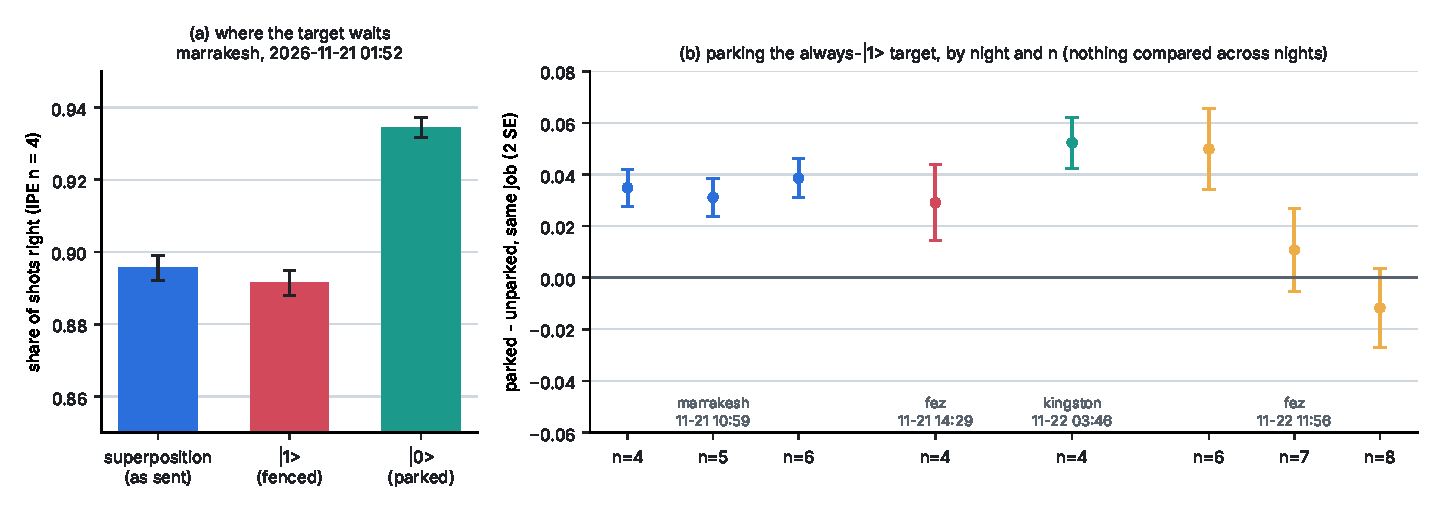
\includegraphics[width=\linewidth]{fig_park.pdf}
\caption{(a) The IPE target waiting in a superposition, in $\ket{1}$ and in $\ket{0}$ (same job). (b) Parking the
always-$\ket{1}$ target against its unparked twin in the same job, by night, device and $n$; each night is read on its
own.}\label{fig:park}
\end{figure}

\paragraph{Parking the likely value (RUS chains).} In RUS chains a waiting qubit is rarely in $\ket{1}$ on every
branch; many are entangled. Turning a qubit with $X$ before a wait and $X$ after leaves the circuit's action unchanged
whenever the qubit takes no part in the wait, entangled or not, and replaces its probability $p$ of being in $\ket{1}$
by $1-p$. On ibm\_fez (2026-11-21) we sent four chains three ways in one job: the default (D), every wait fenced (F),
and fenced with every waiting qubit of noiseless $p > 0.5$ turned (M; not the loop's step). Parking on top of the fence kept $+0.0877$
(2 SE 0.0175) on NF and $+0.0140$ (2 SE 0.0117) on P0, SAME on P2 and P3; the full fence itself cost $-0.0453$
(2 SE 0.0116) on P0 and $-0.0243$ (2 SE 0.0180) on P3. The declared reading was ``damping dominates the waits''.
A fence around the parked qubit and the qubits of its wait only, at those waits only (MP), keeps the $X$ pair from
being cancelled without fencing everything. Sent as psf-os 0.3.1's candidate against 0.3.0's default on ibm\_kingston
(2026-11-22), MP kept $+0.0972$ (2 SE 0.0155) on NF and $+0.0247$ (2 SE 0.0085) on P0, and $+0.0094$ (2 SE 0.0100,
SAME) on P3; no arm overshot. The rule declared beforehand (no counted item KEEPS LESS, at least one KEEPS MORE, the IPE
control KEEPS MORE) made parking the likely value the default in 0.3.1. Figure~\ref{fig:rus}.

\begin{figure}[H]\centering
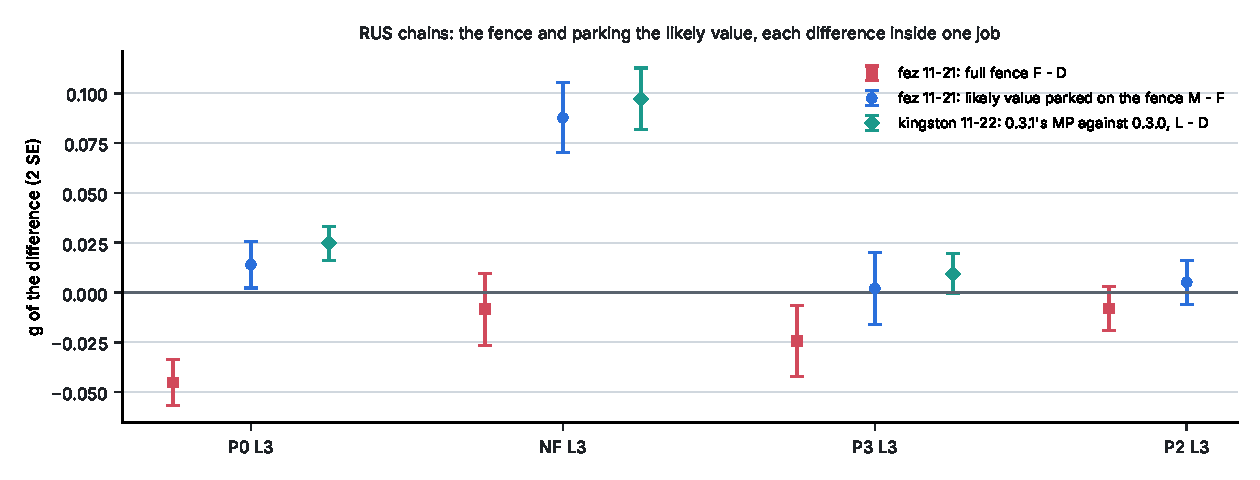
\includegraphics[width=0.86\linewidth]{fig_rus.pdf}
\caption{RUS chains: the full fence (F $-$ D), the likely value parked on the fence (M $-$ F) on ibm\_fez, and 0.3.1's
partial fence against 0.3.0 (L $-$ D) on ibm\_kingston; each difference inside one job.}\label{fig:rus}
\end{figure}

\section{What a wait costs: qubits in superposition and CZ}\label{sec:cost}
A repetition code decoded in real time can be written in forms that differ in how many qubits hold a superposition
while the decision waits (carriers) and how many CZ they use. In one job on marrakesh (2026-11-21, 4000 shots, the four
errors pooled; ceiling 0.875) the four forms read F16 0.7511 (16 CZ, 3 carriers), F10 0.8364 (10, 3), F6P 0.8518 (10, 1)
and F6 0.8741 (6, 1). One carrier instead of three at equal CZ kept $+0.0153$ (2 SE 0.0081); six CZ instead of ten at one
carrier kept $+0.0224$ (2 SE 0.0077); the declared reading: both. F6 stood at the ceiling within its 2 SE but not beyond.
On ibm\_fez (2026-11-21, 1950 shots, a control beside another test) the same comparisons read $+0.0283$ (2 SE 0.0094)
and $+0.0108$ (2 SE 0.0085), and F6 read 0.9294 (2 SE 0.0058), BEYOND THE CEILING. The forms also differ in depth, so a
loss in proportion to time is part of both differences (declared as a limit). F6 undoes the code before the syndrome is read, so that one qubit waits; it cannot protect a memory and is not error
correction. Figure~\ref{fig:wait}.

\begin{figure}[H]\centering
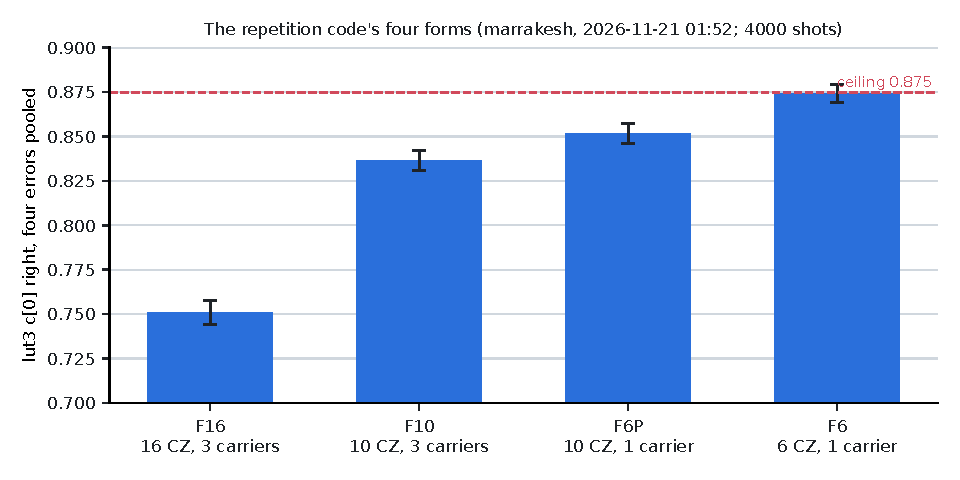
\includegraphics[width=0.62\linewidth]{fig_wait.pdf}
\caption{The repetition code's four forms in one job on marrakesh, with the ceiling.}\label{fig:wait}
\end{figure}

\section{Two conditional items in one circuit}\label{sec:packing}
Paper 10 found that two conditional items packed in one circuit cost the first of them about 0.06, and that the loss
followed the register's bit order: the item whose bits came first lost. A decoy test (2026-11-20, marrakesh) asked
whether that is the register's first bits or the first conditional item, and whether a fixed item placed first
shields the conditional items: in three bundles (no fixed item, the fixed item's bits first, its bits last) the first
conditional item lost $-0.0565$, $-0.0567$ and $-0.085$ against itself alone (2 SE about 0.020), and the second read
SAME everywhere. The declared reading: the first conditional item loses, whatever stands before it. The one declared prediction, that
the control (D0) repeats paper 10's loss, held. psf-os keeps
refusing to pack conditional items side by side.

\section{Deciding inside one job}\label{sec:inside}
\paragraph{Drift between jobs.} The same 40 circuits (the RUS chains of a loop round at $L = 1,2,3$, two copies of every arm, and 4 sentinel circuits) were sent in three jobs, created 8 s apart and finished 40 to 50 s apart (2026-11-20, marrakesh). Copies inside a job agreed (nine pairs
pooled, $\chi^2 = 7.11$ on 9 degrees of freedom, $p = 0.625$). Between jobs, $L = 2$ moved beyond shot noise
($p = 0.006$, an excess standard deviation of 0.014; $g$ changed sign), while $L = 1$ ($p = 0.080$) and $L = 3$
($p = 0.623$) did not. A loop that compares round $k$ with round $k-1$ across jobs can read such a drift as a
prescription's effect. Figure~\ref{fig:loopvar}.

\begin{figure}[H]\centering
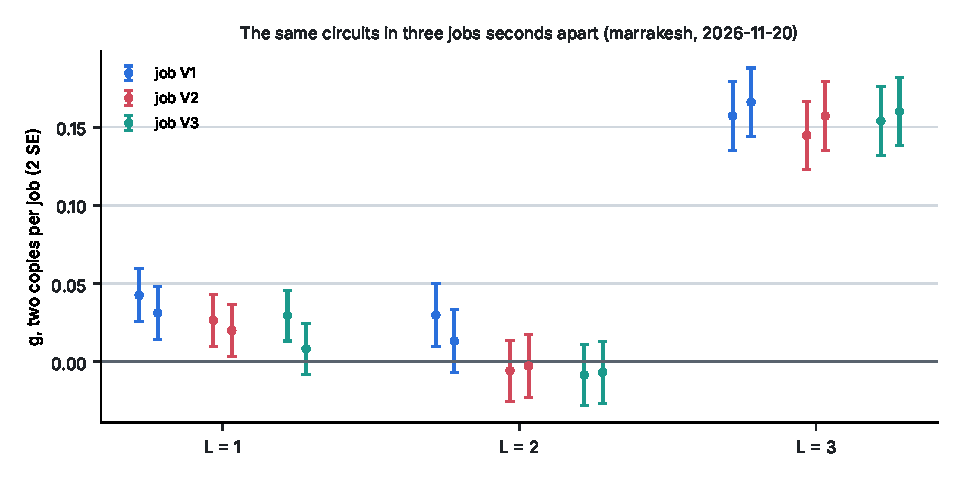
\includegraphics[width=0.62\linewidth]{fig_loopvar.pdf}
\caption{$g$ of the same circuits in three jobs, two copies each.}\label{fig:loopvar}
\end{figure}

\paragraph{The paired loop.} psf-os's loop now places the incumbent prescription and the candidate in the same job and
decides on their difference there. Run on marrakesh (2026-11-20, fetched 14:11 CET, 110 s, unattended), it adopted P2 on $L = 3$
($+0.0388$, 2 SE 0.0215); on $L = 1$ it kept the incumbent against P2 ($+0.0145$, 2 SE 0.0154), tried P2+M in the
next round and adopted it ($+0.0463$, 2 SE 0.0150); it rejected P1 on $L = 2$ ($-0.0225$, 2 SE 0.0194) and added one more try (M) on $L = 3$
($+0.0330$, 2 SE 0.0210). No candidate overshot. The declared prediction (no adopted step overshoots in the next round)
held on the one row it could be read on.

\section{Phase estimation further}\label{sec:ipe}
\paragraph{To $n = 6$.} Unparked IPE on marrakesh (2026-11-21) read 0.8957, 0.8715 and 0.8451 at $n = 4,5,6$, beyond
$C(n)$ by $+0.425$, $+0.492$, $+0.539$. On the log of the share, the loss per added bit was $0.0274$ and $0.0308$; the
acceleration $+0.0034$ (2 SE 0.0077) read FLAT: on this night the loss per added bit did not grow with the conditionals (from 9 to 20) beyond 2 SE.

\paragraph{To $n = 8$, parked.} With psf-os 0.3.1's defaults on ibm\_fez (2026-11-22; 16 phases per $n$ chosen as
$k\cdot a \bmod 2^n$ so that their compiled CZ mix is close to that of every phase), the parked IPE read 0.5785, 0.5097 and 0.4236 at
$n = 6,7,8$, beyond $C(n)$ by $+0.272$, $+0.262$, $+0.223$. The declared reading: the range reaches $n = 8$; parking's gain
is not seen at $n = 8$ at this shot noise. Beside, the loss per added bit grew ($0.1266$ then $0.1851$, acceleration
$+0.0584$, 2 SE 0.0276). On another device and night, from $n = 6$ to 8, it grew; the two ranges are read on their own. The declared
expectation, extrapolated from the marrakesh night, was 0.72; the fez night read 0.4236 (another device and
calibration; set beside, not compared). Figure~\ref{fig:ipe}.

\begin{figure}[H]\centering
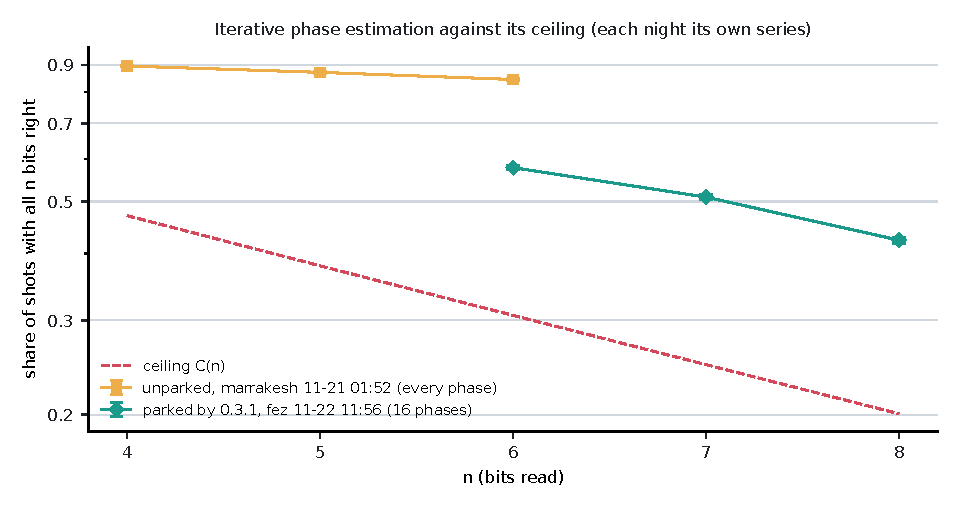
\includegraphics[width=0.62\linewidth]{fig_ipe.pdf}
\caption{IPE share against $n$ on a log scale, each night its own series, with the ceiling $C(n)$.}\label{fig:ipe}
\end{figure}

\paragraph{What the feedback costs.} A test (2026-11-22, fez) sent IPE at $n = 6$ and 8 with the feedback (F), with the
right corrections fixed and unconditional (S), and with S plus a delay of $L$ and $2L$ per removed conditional, to split
the feedback's cost into the branch and its wait. $L$ was declared as 4500 dt before dt was known; read at run time, dt
is 4 ns and $L$ is 18 \textmu s per conditional, and the delayed arms collapsed (0.1177 at $n = 6$ and 0.0494 at $n = 8$, at $L$). The declared
table's row was ``the delay overstates F's wait'': the split is not read from this night. Beside, S $-$ F (the phase conditionals replaced by their right corrections, with the measurement waits kept) changed
the share by $+0.0067$ (2 SE 0.0073) at $n = 6$ and $+0.0023$ (2 SE 0.0083)
at $n = 8$, mean $+0.0045$ (2 SE 0.0055): not separated from 0; the upper end of 2 SE is about $+0.01$.

\section{The operating layer after these tests}\label{sec:psfos}
psf-os 0.3.0 (2026-11-21, doi:10.5281/zenodo.24416958) parks a waiting qubit that is in $\ket{1}$ on every branch, by
default, and records at every build the qubits holding a superposition at each wait. psf-os 0.3.1 (2026-11-22,
doi:10.5281/zenodo.24438701) also parks a waiting qubit whose noiseless probability of $\ket{1}$ is above 0.5, behind a
fence on that qubit and its wait only. Both refuse a build whose noiseless output or compiled CZ count changes, keep
recorded builds as they were built, and refuse a build declared on an earlier version unless the parking is stated. The loop decides inside one job (opt-in up to 0.3.2), and a recorded night can be replayed from its raw counts: with a
ledger line of the same calibration it starts from the ledger's prescriptions, and it stops at the first circuit that
no recorded job holds. psf-os 0.3.3, released with this paper \pending{DOI}, includes 0.3.2 (tagged, not released on its own), which records the
device's time step and prices delays: the branch-cost night's charge was 112 s against a model of 59.6 s, and the model
with the delays' term gives 114.4 s; a delay over 100 \textmu s per circuit is refused unless stated. 0.3.3 follows every
compiled circuit noiselessly through its waits, branch by branch, and refuses a build whose parked qubit did not stay
parked as sent; it records the waits, the fences' cost in depth and a summary of every circuit as sent; it reads the
device's lengths of time (no error number) and refuses a delay off the device's time grid; and on the device it decides
a loop inside one job by default, a decision across jobs having to be stated. Rebuilt with 0.3.3, the test circuits of the six recorded nights of 2026-11-21 and 22 were the same as recorded, gate
for gate and byte for byte, and every wait of a qubit psf-os parked (2214) stayed parked in the circuit as sent. A candidate is now named \texttt{X.Y.ZrcN} until it is released.

\section{What did not work}\label{sec:failed}
The branch-cost split failed because of a placeholder: a delay length declared in device units before the unit was read. It was charged 112 s, 1.9 times the model, because delays were charged and not modelled. The expectation for $n = 8$, extrapolated from another device and night, was 0.72; the night read 0.4236. Parking's gain was not seen at $n = 7$ and 8 on four twin phases. A declaration rule now requires
physical units to be converted with the device's own values before a test is declared, and a delay over 100 \textmu s
per circuit is refused unless stated. Two departures from declarations: the paired loop's declared flags
(\texttt{--k-max 4 --budget 240}) were refused on a device run and it ran without them, with the same values; the $n = 6,7,8$
tool printed its reading from the draft's table, and the record gives the declared table's row.

\section{Limits}\label{sec:limits}
Each rule rests on few nights: parking the always-$\ket{1}$ target on five nights and three devices, parking the
likely value with the partial fence on one night and one device, the repetition code's forms on two. The circuit
families are IPE, RUS chains and a repetition code. The repetition code's forms differ in depth as well as in carriers
and CZ. The drift between jobs was measured on one night, and the packing loss and the drift on one device
(marrakesh). Parking the likely value was read on three chains, one of them SAME. The 8 paired phases of the parked IPE
are cut to fewer CZ by the compiler (6.0 on average at $n = 4$ against 8.0 on the other phases); a phase and its twin
have the same compiled CZ, but parking's gain there was measured on those phases. The unparked IPE's shape to $n = 6$
was read from two jobs. In the shared test of 2026-11-21 the off and floor arms were not sent, because no verdict read them. The paired
loop's prediction was read on one row. Each verdict is read on its own at 2 SE, with no correction for multiple comparisons: the rules rest on the declared
predictions and readings, and no beside value is read on its own (two lie near the line: P0's M $-$ F, $+0.0140$
against 2 SE 0.0117, and the acceleration from $n = 6$ to 8, about 2.1 SE). A peak of errors at one round of IPE on one fez night,
found after the declarations, did not appear on the next fez night with other qubits; it is not used. Values across
nights and devices are set beside each other only.

\section{Reproduction}\label{sec:repro}
Every device result re-scores from its committed raw counts with \texttt{python reproduce.py} in
\texttt{psf-os-lab-notebook}, with the psf-os named in each folder; each folder's README records the re-score SAME at
home and an independent re-count from the raw counts with qiskit, aer and numpy only. The numbers in the records'
READMEs were checked by machine against the score files (\texttt{tools/check\_readme\_numbers.py}, no mismatch over the 66 recorded nights on 2026-11-24). The device runs used qiskit 2.5.2, qiskit-aer 0.17.2 and qiskit-ibm-runtime 0.49.0 (each folder's
\texttt{versions.txt}). Figures: \texttt{notes/paper11/figures.py}; every plotted value, with its source, is in
\texttt{fig\_data.csv}, archived with this paper. The runs are in Table~\ref{tab:runs}.

\begin{table}[H]\centering\footnotesize
\setlength{\tabcolsep}{3.5pt}
\begin{tabular}{llll}
\toprule
fetch (CET) & device & test (results/) & declared predictions \\
\midrule
11-20 11:38 & marrakesh & decoy-night-2026-11-20 & D0: A keeps less packed (the control repeats): held \\
11-20 11:38 & marrakesh & loopvar-night-2026-11-20 & copies agree inside a job: held \\
11-20 14:11 & marrakesh & loop-paired-night-2026-11-20 & no adopted step overshoots next round: held \\
11-21 01:52 & marrakesh & weekend-shared-night-2026-11-21 & F16 not beyond; IPE $n=4$ beyond: both held \\
11-21 10:59 & marrakesh & qpe-parked-night-2026-11-21 & parking keeps more at $n=4$; beyond at $n=4,5,6$: both held \\
11-21 14:29 & fez & rus-fence-night-2026-11-21 & IPE control keeps more: held \\
11-22 03:46 & kingston & likely-park-night-2026-11-22 & control keeps more; NF keeps more: both held \\
11-22 11:56 & fez & qpe-n78-night-2026-11-22 & parked IPE beyond at $n=6$: held \\
11-22 12:55 & fez & ipe-branch-cost-night-2026-11-22 & none declared \\
\bottomrule
\end{tabular}
\caption{The device runs of this paper (charged 165, 110, 111, 83, 48, 40, 37, 112 s; the decoy and loopvar tests
share the 165 s). Over all nights of the series from 11-16 to 11-22: 68 declared, 48 held, 20 failed (the failures are in paper
10).}\label{tab:runs}
\end{table}

\begin{table}[H]\centering\footnotesize
\setlength{\tabcolsep}{3.5pt}
\newcolumntype{R}[1]{>{\raggedright\arraybackslash}p{#1}}
\begin{tabular}{R{3.4cm}lR{2.4cm}R{2.2cm}R{3.3cm}R{2.8cm}}
\toprule
rule & nights & devices & circuits & KEEPS MORE (or the effect) & SAME WITHIN ERROR \\
\midrule
park the always-$\ket{1}$ waiting qubit & 5 & marrakesh, fez, kingston & IPE & $+0.029$ to $+0.052$ & $n = 7, 8$ (fez); the fence in $\ket{1}$ \\
park the likely-$\ket{1}$ waiting qubit & 2 & fez, kingston & RUS chains & $+0.014$ to $+0.097$ & P2, P3 (fez); P3 (kingston) \\
fewer carriers, fewer CZ & 2 & marrakesh, fez & repetition code & $+0.011$ to $+0.028$ & none \\
no conditional items side by side & 1 & marrakesh & RUS items & first item $-0.057$ to $-0.085$ & the second item \\
decide inside one job & 2 & marrakesh & RUS chains & drift between jobs at $L = 2$ ($p = 0.006$) & $L = 1, 3$; copies in a job \\
\bottomrule
\end{tabular}
\caption{The rules and what they rest on (the nights of 2026-11-20 to 22). Each comparison is inside one job; the
drift of the last row is between jobs by design.}\label{tab:rules}
\end{table}

\section{Conclusion}
Table~\ref{tab:rules} gathers the rules and what they rest on. Where a qubit waits changed what a dynamic circuit
kept by up to $+0.10$ in these tests ($+0.014$ to $+0.097$ where it
read KEEPS MORE; SAME WITHIN ERROR on some chains and at $n = 7, 8$). Turning a waiting qubit
that was in $\ket{1}$ on every branch to $\ket{0}$ kept more on three devices; turning one that was only more likely in
$\ket{1}$ kept more than the previous default on one night and one device, on two of three chains. Neither cost CZ nor changed the noiseless answer, which every build checks. Fewer qubits in superposition during a wait and fewer CZ each
kept more. Packed side by side, the first conditional item lost 0.057 to 0.085; psf-os keeps refusing to pack them.
Because the device drifts between jobs, every rule was decided inside one job. Parking is now the default of psf-os;
the paired loop is the default on the device from 0.3.3. Phase estimation, built by those defaults, stayed above its ceiling to eight
bits; removing its phase feedback changed the share by $+0.0045$ (2 SE 0.0055) on the one night it was tried.

\section*{Data and code}
Records, declarations and raw counts: \url{https://github.com/TN-Holdings-LLC/psf-os-lab-notebook}; the operating layer:
\url{https://github.com/TN-Holdings-LLC/psf-os} (releases 0.3.0, doi:10.5281/zenodo.24416958; 0.3.1, doi:10.5281/zenodo.24438701; 0.3.3, which includes 0.3.2, \pending{DOI}).

\section*{References}
\begin{itemize}
\item Smith, K.\ N.\ et al. TimeStitch: exploiting slack to mitigate decoherence in quantum circuits. ACM Trans.\ Quantum
Comput.\ 4(1) (also arXiv:2105.01760, 2021).
\item Liu, H.\ M.\ et al. Idling error suppression through gate scheduling. arXiv:2607.02031 (2026).
\item Zhong, M.\ et al. MERA: a mid-circuit-measurement error-aware compilation framework for quantum circuits. arXiv:2511.10921
(2025).
\item Hothem, D.\ et al. Measuring error rates of mid-circuit measurements. arXiv:2410.16706 (2024).
\item Gaebler, J.\ P.\ et al. Suppression of mid-circuit measurement crosstalk errors with micromotion.
arXiv:2108.10932 (2021).
\item C\'orcoles, A.\ D.\ et al. Exploiting dynamic quantum circuits in a quantum algorithm with superconducting qubits.
Phys.\ Rev.\ Lett.\ 127, 100501 (2021).
\item Cao, Y.\ et al. Quantum neuron. arXiv:1711.11240 (2017).
\item TN Holdings. Papers 7, 8, 9 and 10 of this series: doi:10.5281/zenodo.24046673, 24136512, 24278888, 24367001.
\end{itemize}

\end{document}
